This section will survey some of the most important concurrent models of computation. Before diving into the models, we will first discuss the mathematical semantics\footnote{Nowadays we call these semantics denotational} of computation by Scott.

\begin{figure}[h]
	\centering
   \resizebox{0.95\textwidth}{!}{
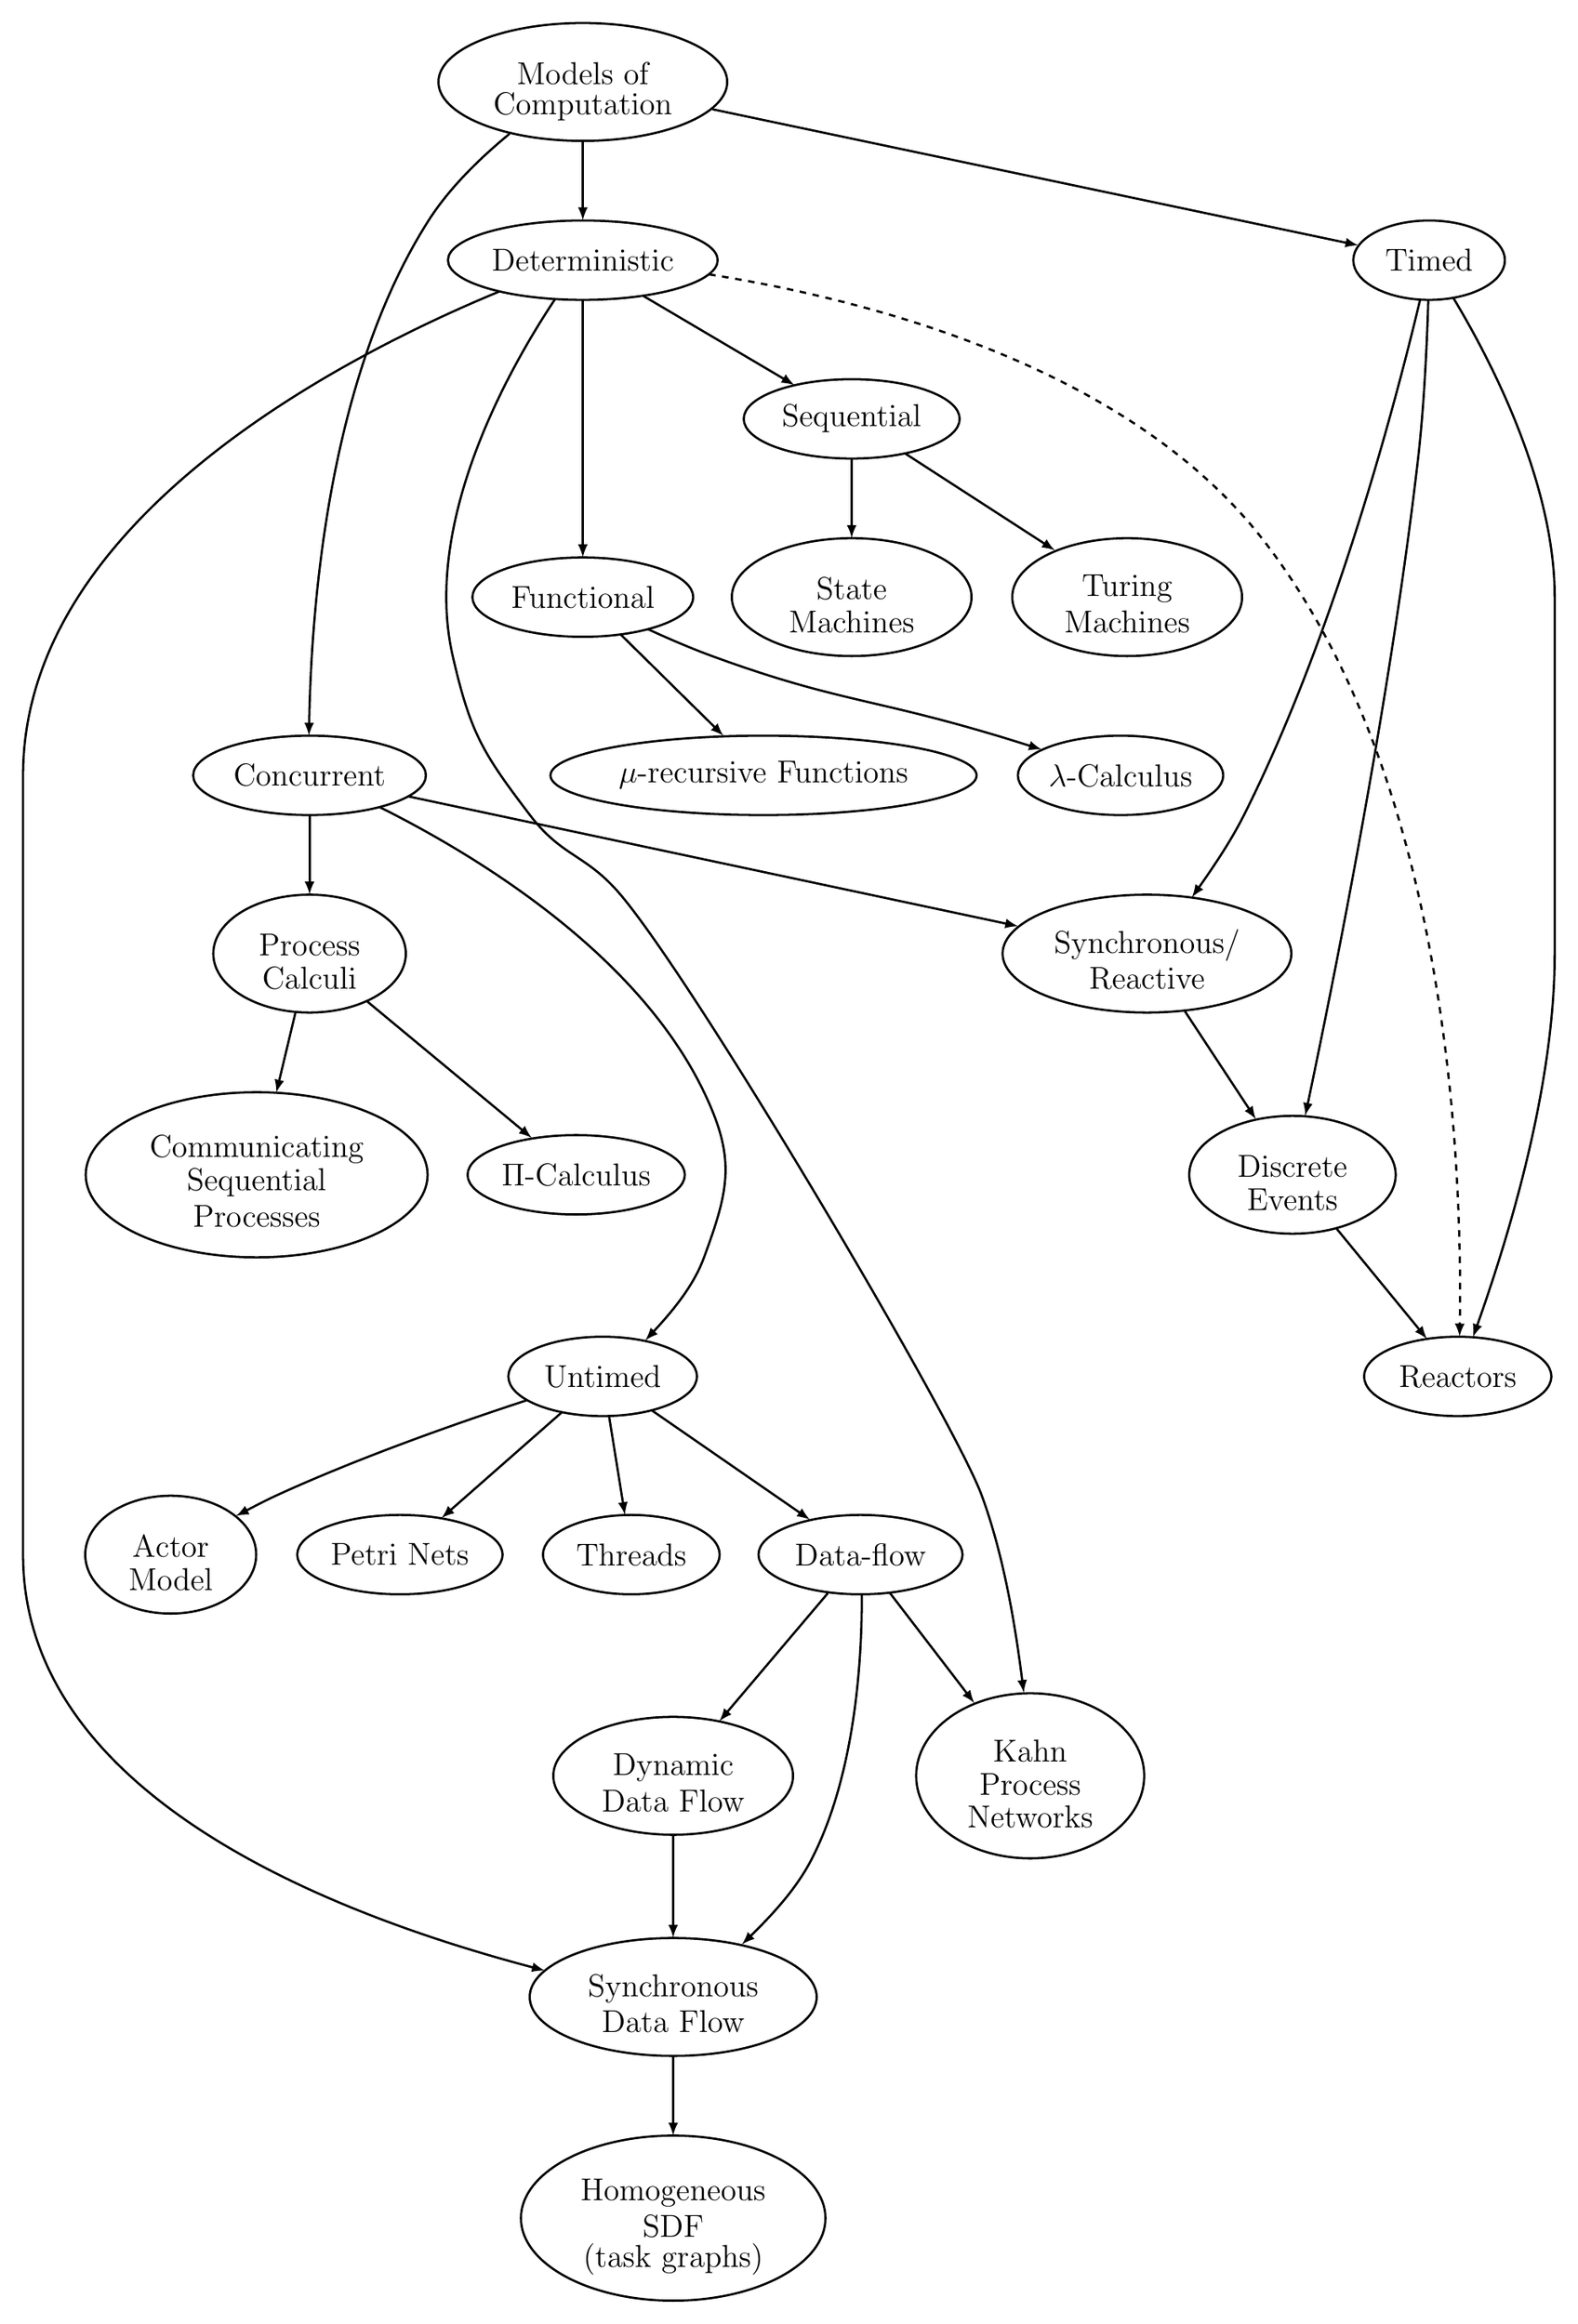
\begin{tikzpicture}[>=latex,line join=bevel,]
  \pgfsetlinewidth{1bp}
\Large%
\pgfsetcolor{black}
  % Edge: root -> concurrent
  \draw [->] (220.74bp,983.16bp) .. controls (207.69bp,972.46bp) and (193.57bp,958.83bp)  .. (184.0bp,943.82bp) .. controls (138.64bp,872.7bp) and (130.81bp,769.62bp)  .. (129.71bp,710.15bp);
  % Edge: root -> t
  \draw [->] (312.74bp,994.32bp) .. controls (390.88bp,977.86bp) and (527.12bp,949.17bp)  .. (605.85bp,932.59bp);
  % Edge: root -> det
  \draw [->] (254.0bp,979.76bp) .. controls (254.0bp,971.49bp) and (254.0bp,962.37bp)  .. (254.0bp,943.97bp);
  % Edge: seq -> touring
  \draw [->] (400.4bp,838.04bp) .. controls (417.23bp,827.14bp) and (440.03bp,812.4bp)  .. (468.15bp,794.2bp);
  % Edge: seq -> sm
  \draw [->] (376.0bp,835.47bp) .. controls (376.0bp,827.9bp) and (376.0bp,818.84bp)  .. (376.0bp,799.82bp);
  % Edge: concurrent -> ut
  \draw [->] (161.9bp,677.64bp) .. controls (204.61bp,656.31bp) and (278.5bp,611.95bp)  .. (309.0bp,548.34bp) .. controls (323.4bp,518.3bp) and (320.51bp,504.65bp)  .. (309.0bp,473.39bp) .. controls (304.9bp,462.24bp) and (297.35bp,451.82bp)  .. (282.39bp,435.75bp);
  % Edge: concurrent -> pc
  \draw [->] (130.0bp,673.73bp) .. controls (130.0bp,666.16bp) and (130.0bp,657.1bp)  .. (130.0bp,638.08bp);
  % Edge: concurrent -> sr
  \draw [->] (174.71bp,682.57bp) .. controls (240.52bp,668.56bp) and (364.01bp,642.28bp)  .. (451.49bp,623.66bp);
  % Edge: t -> sr
  \draw [->] (633.88bp,907.73bp) .. controls (623.81bp,865.35bp) and (595.74bp,757.01bp)  .. (554.0bp,674.08bp) .. controls (549.05bp,664.25bp) and (542.72bp,654.22bp)  .. (530.4bp,636.76bp);
  % Edge: t -> de
  \draw [->] (637.62bp,907.5bp) .. controls (637.08bp,889.27bp) and (635.84bp,860.54bp)  .. (633.0bp,835.82bp) .. controls (620.89bp,730.61bp) and (596.54bp,607.86bp)  .. (581.81bp,537.67bp);
  % Edge: t -> reactors
  \draw [->] (648.99bp,908.71bp) .. controls (665.55bp,881.24bp) and (695.0bp,825.07bp)  .. (695.0bp,772.95bp) .. controls (695.0bp,772.95bp) and (695.0bp,772.95bp)  .. (695.0bp,611.21bp) .. controls (695.0bp,551.4bp) and (674.43bp,483.7bp)  .. (657.97bp,437.32bp);
  % Edge: ut -> petri
  \draw [->] (244.38bp,403.02bp) .. controls (231.0bp,391.26bp) and (212.77bp,375.23bp)  .. (189.91bp,355.14bp);
  % Edge: ut -> df
  \draw [->] (285.28bp,403.99bp) .. controls (303.19bp,391.61bp) and (328.55bp,374.08bp)  .. (357.0bp,354.41bp);
  % Edge: ut -> threads
  \draw [->] (265.95bp,401.04bp) .. controls (267.59bp,390.83bp) and (269.67bp,377.92bp)  .. (273.11bp,356.52bp);
  % Edge: ut -> actors
  \draw [->] (228.58bp,408.57bp) .. controls (198.18bp,398.61bp) and (152.91bp,382.78bp)  .. (115.0bp,365.39bp) .. controls (111.87bp,363.95bp) and (108.66bp,362.38bp)  .. (96.573bp,356.04bp);
  % Edge: det -> seq
  \draw [->] (281.38bp,909.66bp) .. controls (299.09bp,899.21bp) and (322.3bp,885.51bp)  .. (349.97bp,869.18bp);
  % Edge: det -> f
  \draw [->] (254.0bp,907.68bp) .. controls (254.0bp,881.37bp) and (254.0bp,832.34bp)  .. (254.0bp,791.06bp);
  % Edge: det -> sdf
  \draw [->] (215.97bp,911.56bp) .. controls (145.12bp,882.24bp) and (0.0bp,808.04bp)  .. (0.0bp,692.08bp) .. controls (0.0bp,692.08bp) and (0.0bp,692.08bp)  .. (0.0bp,338.52bp) .. controls (0.0bp,229.37bp) and (139.76bp,175.39bp)  .. (236.72bp,149.82bp);
  % Edge: det -> kpn
  \draw [->] (241.3bp,908.01bp) .. controls (220.08bp,876.08bp) and (181.04bp,806.73bp)  .. (195.0bp,746.08bp) .. controls (202.98bp,711.41bp) and (208.43bp,702.38bp)  .. (230.0bp,674.08bp) .. controls (244.7bp,654.8bp) and (255.3bp,656.56bp)  .. (271.0bp,638.08bp) .. controls (305.71bp,597.21bp) and (422.24bp,400.09bp)  .. (435.0bp,365.39bp) .. controls (444.34bp,339.98bp) and (449.76bp,310.24bp)  .. (454.09bp,275.83bp);
  % Edge: det -> reactors
  \draw [->,dashed] (311.3bp,919.38bp) .. controls (382.04bp,908.19bp) and (500.51bp,878.25bp)  .. (562.0bp,799.82bp) .. controls (646.84bp,691.61bp) and (653.12bp,516.23bp)  .. (651.83bp,437.52bp);
  % Edge: f -> mu
  \draw [->] (271.39bp,755.8bp) .. controls (282.79bp,744.56bp) and (297.88bp,729.68bp)  .. (317.78bp,710.05bp);
  % Edge: f -> l
  \draw [->] (283.64bp,758.37bp) .. controls (292.92bp,754.1bp) and (303.27bp,749.63bp)  .. (313.0bp,746.08bp) .. controls (368.92bp,725.68bp) and (384.99bp,727.19bp)  .. (442.0bp,710.08bp) .. controls (445.38bp,709.07bp) and (448.87bp,708.0bp)  .. (462.22bp,703.81bp);
  % Edge: pc -> pic
  \draw [->] (156.26bp,589.44bp) .. controls (175.93bp,573.12bp) and (202.8bp,550.84bp)  .. (230.79bp,527.63bp);
  % Edge: pc -> csp
  \draw [->] (123.63bp,584.58bp) .. controls (121.67bp,576.4bp) and (119.46bp,567.13bp)  .. (114.93bp,548.19bp);
  % Edge: df -> sdf
  \draw [->] (380.58bp,320.47bp) .. controls (380.72bp,293.06bp) and (378.06bp,239.96bp)  .. (358.0bp,200.69bp) .. controls (352.01bp,188.97bp) and (343.03bp,178.08bp)  .. (326.21bp,161.67bp);
  % Edge: df -> ddf
  \draw [->] (365.19bp,321.04bp) .. controls (353.5bp,307.24bp) and (336.86bp,287.59bp)  .. (316.0bp,262.97bp);
  % Edge: df -> kpn
  \draw [->] (393.41bp,321.04bp) .. controls (402.28bp,309.48bp) and (414.3bp,293.82bp)  .. (431.61bp,271.25bp);
  % Edge: sdf -> tg
  \draw [->] (295.0bp,110.93bp) .. controls (295.0bp,103.0bp) and (295.0bp,94.08bp)  .. (295.0bp,75.005bp);
  % Edge: ddf -> sdf
  \draw [->] (295.0bp,211.28bp) .. controls (295.0bp,200.14bp) and (295.0bp,187.04bp)  .. (295.0bp,164.79bp);
  % Edge: sr -> de
  \draw [->] (527.17bp,585.11bp) .. controls (535.31bp,572.72bp) and (545.15bp,557.77bp)  .. (559.37bp,536.14bp);
  % Edge: de -> reactors
  \draw [->] (596.1bp,486.35bp) .. controls (606.71bp,473.41bp) and (619.7bp,457.56bp)  .. (637.02bp,436.44bp);
  % Node: root
\begin{scope}
  \definecolor{strokecol}{rgb}{0.0,0.0,0.0};
  \pgfsetstrokecolor{strokecol}
  \draw (254.0bp,1006.69bp) ellipse (65.52bp and 26.74bp);
  \draw (254.0bp,1010.49bp) node {Models of };
  \draw (254.0bp,995.49bp) node { Computation};
\end{scope}
  % Node: concurrent
\begin{scope}
  \definecolor{strokecol}{rgb}{0.0,0.0,0.0};
  \pgfsetstrokecolor{strokecol}
  \draw (130.0bp,692.08bp) ellipse (52.79bp and 18.0bp);
  \draw (130.0bp,692.08bp) node {Concurrent};
\end{scope}
  % Node: t
\begin{scope}
  \definecolor{strokecol}{rgb}{0.0,0.0,0.0};
  \pgfsetstrokecolor{strokecol}
  \draw (638.0bp,925.82bp) ellipse (34.39bp and 18.0bp);
  \draw (638.0bp,925.82bp) node {Timed};
\end{scope}
  % Node: det
\begin{scope}
  \definecolor{strokecol}{rgb}{0.0,0.0,0.0};
  \pgfsetstrokecolor{strokecol}
  \draw (254.0bp,925.82bp) ellipse (61.19bp and 18.0bp);
  \draw (254.0bp,925.82bp) node {Deterministic};
\end{scope}
  % Node: seq
\begin{scope}
  \definecolor{strokecol}{rgb}{0.0,0.0,0.0};
  \pgfsetstrokecolor{strokecol}
  \draw (376.0bp,853.82bp) ellipse (48.99bp and 18.0bp);
  \draw (376.0bp,853.82bp) node {Sequential};
\end{scope}
  % Node: f
\begin{scope}
  \definecolor{strokecol}{rgb}{0.0,0.0,0.0};
  \pgfsetstrokecolor{strokecol}
  \draw (254.0bp,772.95bp) ellipse (50.09bp and 18.0bp);
  \draw (254.0bp,772.95bp) node {Functional};
\end{scope}
  % Node: touring
\begin{scope}
  \definecolor{strokecol}{rgb}{0.0,0.0,0.0};
  \pgfsetstrokecolor{strokecol}
  \draw (501.0bp,772.95bp) ellipse (52.15bp and 26.74bp);
  \draw (501.0bp,776.75bp) node {Turing };
  \draw (501.0bp,761.75bp) node { Machines};
\end{scope}
  % Node: sm
\begin{scope}
  \definecolor{strokecol}{rgb}{0.0,0.0,0.0};
  \pgfsetstrokecolor{strokecol}
  \draw (376.0bp,772.95bp) ellipse (54.39bp and 26.74bp);
  \draw (376.0bp,776.75bp) node {State };
  \draw (376.0bp,761.75bp) node {  Machines};
\end{scope}
  % Node: ut
\begin{scope}
  \definecolor{strokecol}{rgb}{0.0,0.0,0.0};
  \pgfsetstrokecolor{strokecol}
  \draw (263.0bp,419.39bp) ellipse (42.79bp and 18.0bp);
  \draw (263.0bp,419.39bp) node {Untimed};
\end{scope}
  % Node: pc
\begin{scope}
  \definecolor{strokecol}{rgb}{0.0,0.0,0.0};
  \pgfsetstrokecolor{strokecol}
  \draw (130.0bp,611.21bp) ellipse (43.68bp and 26.74bp);
  \draw (130.0bp,615.01bp) node {Process };
  \draw (130.0bp,600.01bp) node { Calculi};
\end{scope}
  % Node: sr
\begin{scope}
  \definecolor{strokecol}{rgb}{0.0,0.0,0.0};
  \pgfsetstrokecolor{strokecol}
  \draw (510.0bp,611.21bp) ellipse (65.52bp and 26.74bp);
  \draw (510.0bp,615.01bp) node {Synchronous/};
  \draw (510.0bp,600.01bp) node { Reactive};
\end{scope}
  % Node: kpn
\begin{scope}
  \definecolor{strokecol}{rgb}{0.0,0.0,0.0};
  \pgfsetstrokecolor{strokecol}
  \draw (457.0bp,238.17bp) ellipse (51.74bp and 37.45bp);
  \draw (457.0bp,249.47bp) node {Kahn };
  \draw (457.0bp,234.47bp) node { Process };
  \draw (457.0bp,219.47bp) node { Networks};
\end{scope}
  % Node: de
\begin{scope}
  \definecolor{strokecol}{rgb}{0.0,0.0,0.0};
  \pgfsetstrokecolor{strokecol}
  \draw (576.0bp,510.86bp) ellipse (46.84bp and 26.74bp);
  \draw (576.0bp,514.66bp) node {Discrete };
  \draw (576.0bp,499.66bp) node { Events};
\end{scope}
  % Node: reactors
\begin{scope}
  \definecolor{strokecol}{rgb}{0.0,0.0,0.0};
  \pgfsetstrokecolor{strokecol}
  \draw (651.0bp,419.39bp) ellipse (42.49bp and 18.0bp);
  \draw (651.0bp,419.39bp) node {Reactors};
\end{scope}
  % Node: petri
\begin{scope}
  \definecolor{strokecol}{rgb}{0.0,0.0,0.0};
  \pgfsetstrokecolor{strokecol}
  \draw (171.0bp,338.52bp) ellipse (46.59bp and 18.0bp);
  \draw (171.0bp,338.52bp) node {Petri Nets};
\end{scope}
  % Node: df
\begin{scope}
  \definecolor{strokecol}{rgb}{0.0,0.0,0.0};
  \pgfsetstrokecolor{strokecol}
  \draw (380.0bp,338.52bp) ellipse (46.29bp and 18.0bp);
  \draw (380.0bp,338.52bp) node {Data-flow};
\end{scope}
  % Node: threads
\begin{scope}
  \definecolor{strokecol}{rgb}{0.0,0.0,0.0};
  \pgfsetstrokecolor{strokecol}
  \draw (276.0bp,338.52bp) ellipse (40.09bp and 18.0bp);
  \draw (276.0bp,338.52bp) node {Threads};
\end{scope}
  % Node: actors
\begin{scope}
  \definecolor{strokecol}{rgb}{0.0,0.0,0.0};
  \pgfsetstrokecolor{strokecol}
  \draw (67.0bp,338.52bp) ellipse (38.78bp and 26.74bp);
  \draw (67.0bp,342.32bp) node {Actor };
  \draw (67.0bp,327.32bp) node { Model};
\end{scope}
  % Node: sdf
\begin{scope}
  \definecolor{strokecol}{rgb}{0.0,0.0,0.0};
  \pgfsetstrokecolor{strokecol}
  \draw (295.0bp,137.82bp) ellipse (65.11bp and 26.74bp);
  \draw (295.0bp,141.62bp) node {Synchronous };
  \draw (295.0bp,126.62bp) node { Data Flow};
\end{scope}
  % Node: mu
\begin{scope}
  \definecolor{strokecol}{rgb}{0.0,0.0,0.0};
  \pgfsetstrokecolor{strokecol}
  \draw (336.0bp,692.08bp) ellipse (96.68bp and 18.0bp);
  \draw (336.0bp,692.08bp) node {$\mu$-recursive Functions};
\end{scope}
  % Node: l
\begin{scope}
  \definecolor{strokecol}{rgb}{0.0,0.0,0.0};
  \pgfsetstrokecolor{strokecol}
  \draw (498.0bp,692.08bp) ellipse (46.59bp and 18.0bp);
  \draw (498.0bp,692.08bp) node {$\lambda$-Calculus};
\end{scope}
  % Node: pic
\begin{scope}
  \definecolor{strokecol}{rgb}{0.0,0.0,0.0};
  \pgfsetstrokecolor{strokecol}
  \draw (251.0bp,510.86bp) ellipse (49.29bp and 18.0bp);
  \draw (251.0bp,510.86bp) node {$\Pi$-Calculus};
\end{scope}
  % Node: csp
\begin{scope}
  \definecolor{strokecol}{rgb}{0.0,0.0,0.0};
  \pgfsetstrokecolor{strokecol}
  \draw (106.0bp,510.86bp) ellipse (77.56bp and 37.45bp);
  \draw (106.0bp,522.16bp) node {Communicating };
  \draw (106.0bp,507.16bp) node { Sequential  };
  \draw (106.0bp,492.16bp) node { Processes};
\end{scope}
  % Node: ddf
\begin{scope}
  \definecolor{strokecol}{rgb}{0.0,0.0,0.0};
  \pgfsetstrokecolor{strokecol}
  \draw (295.0bp,238.17bp) ellipse (54.39bp and 26.74bp);
  \draw (295.0bp,241.97bp) node {Dynamic };
  \draw (295.0bp,226.97bp) node { Data Flow};
\end{scope}
  % Node: tg
\begin{scope}
  \definecolor{strokecol}{rgb}{0.0,0.0,0.0};
  \pgfsetstrokecolor{strokecol}
  \draw (295.0bp,37.48bp) ellipse (69.09bp and 37.45bp);
  \draw (295.0bp,48.78bp) node {Homogeneous };
  \draw (295.0bp,33.78bp) node { SDF };
  \draw (295.0bp,18.78bp) node { (task graphs)};
\end{scope}
%
\end{tikzpicture}
}
	\caption{Overview of different models of computation.}
	\label{fig:dataflow_mocs}
\end{figure}



\subsection{Partial Computation: Scott Domains}

When Dana Scott proposed his mathematical theory of computation~\cite{scott1970}, he used the term mathematical to contrast it with operational computation.
In practice, the steps of a computation are defined by the \ac{ISA} of the machine executing them.
Most people don't write programs directly for the \ac{ISA}, however. They write them in an abstract programming language, which is translated by a compiler into machine instructions.
Thus, in practice, the implementation of a compiler is what defines the (operational) semantics of programs.
Scott's theory had the ambitious goal of being an abstraction that sat between these operational semantics and the abstract notions of computability of e.g. Church or Turing.
He intended to abstract away the arbitrary implementation choices that were necessary but did not change the essence of the execution.
While today his model is not the single established abstract model of semantics he sought out to define, it introduced several important ideas and mathematical structures to models of computation.
In particular, a crucial abstraction introduced by his theory is that of partial computation.
His theory makes it possible to express a computation as a series of partial results, without regarding the actual implementation of these.
We will now introduce the basics of Scott's mathematical theory of computation.


A Domain is a particular type of \ac{poset} ... 

For example ...


Scott's computation model implicitly assumed a sequential computation and Scott-continuous functions are a powerful method for describing partial sequential computations.
Can we also use this model to describe parallel computation?
Gilles Kahn did precisely this, four years after Scott published his mathematical theory of computation. 
He used the formalism of Scott to define a model of parallel computation, based on what he coined as process networks, now known as Kahn Process Networks.

The basic idea to generalize the Scott theory of computation is simple

\begin{figure}[h]
	\centering
   \resizebox{0.55\textwidth}{!}{\begin{tikzpicture}%[fill opacity=0.3]
%circles
\node[ellipse, fill=green!20, minimum width = 9cm,minimum height = 5cm,draw] (ddf) at (0,3) {};
\node[ellipse, fill=green!60, minimum width = 6.2cm,minimum height = 4.5cm,draw] (kpn) at (1,3) {};
\node[ellipse, fill=green!50, minimum width = 5.5cm,minimum height = 4.0cm,draw] (kmq) at (1,2.8) {};
\node[ellipse, fill=green!70, minimum width = 4.8cm,minimum height = 3.5cm,draw] (csdf) at (1,2.6) {};
\node[ellipse, fill=green!30, minimum width = 3cm,minimum height = 3cm,draw] (sdf) at (1.5,2.5) {SDF};
\node[ellipse, fill=green!40, minimum width = 1.0cm,minimum height = 1.0cm,draw] (hsdf) at (1.5,3.4) {HSDF};

%labels
\node (lbl-ddf) at (-3,3) {DDF};
%\node (lbl-sdf) at (0,1.5) {SDF};
%\node (lbl-hsdf) at (0,0) {HSDF};
\node (lbl-kmq) at (1,4.5) {KMQ};
\node (lbl-sadf) at (-0.6,2.5) {CSDF};
\node (lbl-kpn) at (1,5.0) {KPN};
  
\end{tikzpicture}
}
	\caption{Relationships between different dataflow models of computation.}
	\label{fig:dataflow_mocs}
\end{figure}



\subsection{Concurrent Computation: Kahn Process Networks}
Discuss related: Hewitt-Agha actor model\index{actor model}~\cite{DBLP:conf/ijcai/HewittBS73,Agha:86:Actors}, Petri Nets\index{Petri nets}~\cite{petri1962nets}, Process Calculi\index{Process Calculi} (\index{Process Calculi ! Pi-Calculus}$\Pi$-calculus, \index{Process Calculi ! CSP}\ac{CSP})
\index{Kahn Process Networks}\ac{KPN}~\cite{kahn74}

\subsection{Dataflow Models of Computation}
Dennis dataflow \index{Dataflow ! Dennis}~\cite{dennis1974first,dennis1986data}
\cite{Parks:M95/105}
Dataflow process networks~\cite{lee1995dataflow,lee_matsikoudis_semantics}
\ac{CSDF}\index{Dataflow ! CSDF}~\cite{bilsen1996cycle}
\ac{SADF}\index{Dataflow ! SADF}~\cite{theelen2006scenario}
\ac{SDF}\index{Dataflow ! SDF}~\cite{lee1987sdf}



